\documentclass{article}
\usepackage{tikz}
\usepackage{pgfplots}
\pgfplotsset{compat=1.18}

\begin{document}

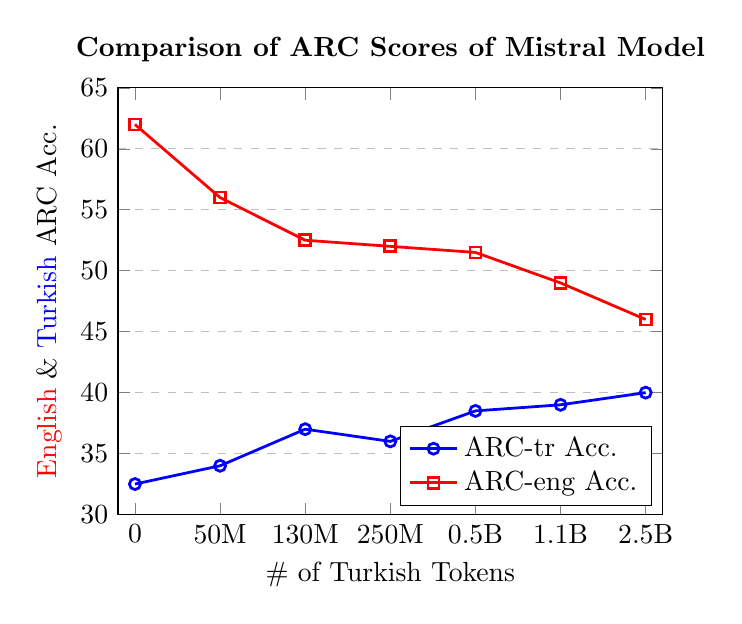
\begin{tikzpicture}
\begin{axis}[
    width=8.5cm,
    height=7cm,
    title={\textbf{Comparison of ARC Scores of Mistral Model}},
    xlabel={\# of Turkish Tokens},
    ylabel={\textcolor{red}{English} \& \textcolor{blue}{Turkish} ARC Acc.},
    xmin=-0.2, xmax=6.2,
    ymin=30, ymax=65,
    xtick={0,1,2,3,4,5,6},
    xticklabels={0,50M,130M,250M,0.5B,1.1B,2.5B},
    ytick={30,35,40,45,50,55,60,65},
    ymajorgrids=true,
    grid style=dashed,
    legend style={at={(0.98,0.02)}, anchor=south east},
    legend cell align={left},
]

% Turkish ARC accuracy data (blue)
\addplot[
    color=blue,
    mark=o,
    line width=1pt,
    ]
    coordinates {
    (0,32.5) (1,34) (2,37) (3,36) (4,38.5) (5,39) (6,40)
    };
    
% English ARC accuracy data (red)
\addplot[
    color=red,
    mark=square,
    line width=1pt,
    ]
    coordinates {
    (0,62) (1,56) (2,52.5) (3,52) (4,51.5) (5,49) (6,46)
    };

\legend{ARC-tr Acc., ARC-eng Acc.}

\end{axis}
\end{tikzpicture}

\end{document}